\documentclass[uplatex, dvipdfmx]{jsarticle}


\usepackage{tcolorbox}
\usepackage{color}
\usepackage{listings, plistings}

%% ノート/latexメモ
%% http://pepper.is.sci.toho-u.ac.jp/pepper/index.php?%A5%CE%A1%BC%A5%C8%2Flatex%A5%E1%A5%E2

%% JavaScriptの設定
%% https://e8l.hatenablog.com/entry/2015/11/29/232800
\lstdefinelanguage{javascript}{
  morekeywords = [1]{ %keywords
    await, break, case, catch, class, const, continue, debugger, default, delete, 
    do, else, enum, export, extends, finally, for, function, function*, if, implements, import, in, 
    instanceof, interface, let, new, package, private, protected, public, return, static, super,
    switch, this, throw, try, typeof, var, void, while, with, yield, yield*
  },
  morekeywords = [2]{ %literal
    false, Infinity, NaN, null, true, undefined
  },
  morekeywords = [3] { %Classes
    Array, ArrayBuffer, Boolean, DataView, Date, Error, EvalError, Float32Array, Float64Array,
    Function, Generator, GeneratorFunction, Int16Array, Int32Array, Int8Array, InternalError,
    JSON, Map, Math, Number, Object, Promise, Proxy, RangeError, ReferenceError, Reflect,
    RegExp, Set, String, Symbol, SyntaxError, TypeError, URIError, Uint16Array, Uint32Array,
    Uint8Array, Uint8ClampedArray, WeakMap, WeakSet
  },
  morecomment = [l]{//},
  morecomment = [s]{/*}{*/},
  morestring = [b]{"},
  morestring = [b]{'},
  alsodigit = {-},
  sensitive = true
}

%% 修正時刻: Tue 2022/03/15 10:04:41


% Java
\lstset{% 
  frame=single,
  backgroundcolor={\color[gray]{.9}},
  stringstyle={\ttfamily \color[rgb]{0,0,1}},
  commentstyle={\itshape \color[cmyk]{1,0,1,0}},
  identifierstyle={\ttfamily}, 
  keywordstyle={\ttfamily \color[cmyk]{0,1,0,0}},
  basicstyle={\ttfamily},
  breaklines=true,
  xleftmargin=0zw,
  xrightmargin=0zw,
  framerule=.2pt,
  columns=[l]{fullflexible},
  numbers=left,
  stepnumber=1,
  numberstyle={\scriptsize},
  numbersep=1em,
  language={Java},
  lineskip=-0.5zw,
  morecomment={[s][{\color[cmyk]{1,0,0,0}}]{/**}{*/}},
  keepspaces=true,         % 空白の連続をそのままで
  showstringspaces=false,  % 空白字をOFF
}
%\usepackage[dvipdfmx]{graphicx}
\usepackage{url}
\usepackage[dvipdfmx]{hyperref}
\usepackage{amsmath, amssymb}
\usepackage{itembkbx}
\usepackage{eclbkbox}	% required for `\breakbox' (yatex added)
\usepackage{enumerate}
\usepackage[default]{cantarell}
\usepackage[T1]{fontenc}
\fboxrule=0.5pt
\parindent=1em
\definecolor{mygrey}{rgb}{0.97, 0.97, 0.97}

\makeatletter
\def\verbatim@font{\normalfont
\let\do\do@noligs
\verbatim@nolig@list}
\makeatother

\begin{document}

%\anaumeと入力すると穴埋め解答欄が作れるようにしてる。\anaumesmallで小さめの穴埋めになる。
\newcounter{mycounter} % カウンターを作る
\setcounter{mycounter}{0} % カウンターを初期化
\newcommand{\anaume}[1][]{\refstepcounter{mycounter}{#1}{\boxed{\phantom{aa}\textnormal{\themycounter}\phantom{aa}}}} %穴埋め問題の空欄作ってる。
\newcommand{\anaumesmall}[1][]{\refstepcounter{mycounter}{#1}{\boxed{\tiny{\phantom{a}\themycounter \phantom{a}}}}}%小さい版作ってる。色々改造できる。

%% 修正時刻: Tue 2022/03/15 10:04:411


\section{MAMPの設定}

\subsection{PHPのバージョン}

MAMPがせっかくPHP8に対応したが、PHP8だとWordPressを動かした場合、
不具合が発生するので、PHP7を動かすことにする。

まず、MAMPを停止させ、MAMPを閉じてから、以下の作業をする。

C:\yen MAMP\yen bin\yen php にある以下のフォルダの名前を変更する。

\vspace{3mm}
\begin{tabular}{|lll|} \hline
php8.0.1 & $\rightarrow$ & \_php8.0.1 \\
php8.1.0 & $\rightarrow$ & \_php8.1.0 \\ \hline
\end{tabular}
\vspace{3mm}

MAMPを起動させる。
PHP のバージョンを確認する。

\vspace{3mm}
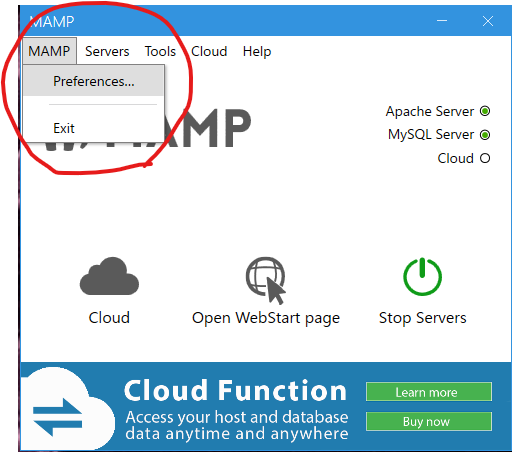
\includegraphics[width=10cm]{img/13-preferences.png}
\vspace{3mm}

ここに選択できるバージョンが示されるので、それを選択する。

\vspace{3mm}
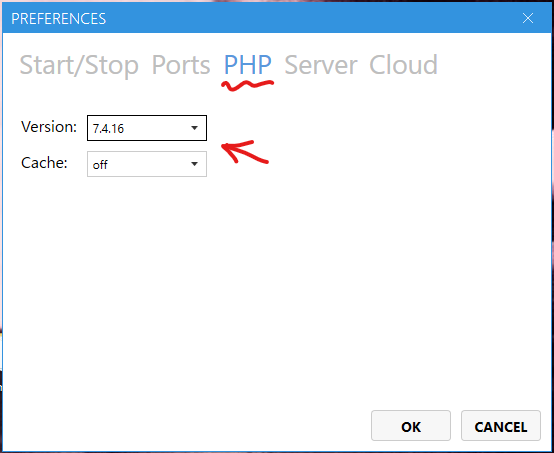
\includegraphics[width=10cm]{img/14-php-ver.png}
\vspace{3mm}

このバージョンは覚えておく。


\subsection{PHPの設定}

PHPの設定ファイルは以下である。(php v7.4.16 の場合)

"C:\yen MAMP\yen conf\yen php7.4.16\yen php.ini"

一応バックアップはとっておく。

\fbox{pnp.ini\_org} という名前でオリジナルファイルは残しておく。

\begin{lstlisting}[caption=php.ini]
307 memory_limit = 512M

375 display_errors = on

494 post_max_size = 512M

518 default_charset = "UTF-8"

607 upload_max_filesize = 512M

705 date.timezone = Asia/Tokyo
\end{lstlisting}

307, 494, 607 を 512M としたのは、今後 WordPress でバックアップファイルから
復元するときのことを考慮したのである。

375 で on とすることにより、エラーがブラウザに出力されるようになる。

518 で UTF-8 と指定しているが、これは指定しなくても UTF-8 になるようである。

705 でタイムゾーンを指定している。これは必須である。

要するに、絶対に指定しなければならないのは、705行めのタイムゾーンだけである。


\subsection{MySQLの設定}

設定ファイルは C:\yen MAMP\yen conf\yen mysql\yen my.ini である。

オリジナルは my.ini\_org としてバックアップしておく。

\begin{lstlisting}[caption=my.ini]
...
40 character-set-server=utf8 
41 collation-server=utf8_general_ci
...
\end{lstlisting}

とあるが、これを以下のようにしておく。

\begin{lstlisting}[caption=my.ini]
...
40 character-set-server=utf8mb4 
41 collation-server=utf8mb4_general_ci
...
\end{lstlisting}

UTF-8の文字コードは本来4バイトなのだが、
MySQLで使われてきたUTF-8は3バイトであった。
そのことにより使用できる文字が制限されてきた。

MySQL5.7.9 以降では UTF-8mb4(4バイト)が使えるようになった。





\end{document}

%% 修正時刻: Sat May  2 15:10:04 2020


%% 修正時刻: Sun 2022/08/21 09:02:202
